% !TEX root = ../main.tex

\chapter{\label{chapitre:contexte}Processeurs multi-cœur et interférences}

L'utilisation de processeurs multi-cœur COTS dans les nouvelles générations de calculateurs est une piste prometteuse pour accompagner la montée en complexité des systèmes embarqués.
Cela pose néanmoins le défi de concilier les exigences de déterminisme propre à des systèmes critiques et temps-réel, et les choix de conception de matériel destiné au marché de masse.
D'une part, les systèmes embarqués temps-réels doivent se conformer à un principe d'isolation temporelle. 
C'est-à-dire que dans un tel système la performance d'une application ne doit pas être affectée par celle des autres.
D'autre part, le matériel que nous souhaitons utiliser étant conçu pour offrir de bonnes performances à bas coût, des composants matériels sont partagés entre les cœurs, altérant ainsi la performance des applications s'exécutant en parallèle.
%Ces \emph{interférences} entrent directement en contradiction avec les 

Dans ce chapitre, nous allons étudier en détail la cause de ces \emph{interférences}. 
Nous commencerons par présenter l'architecture des systèmes embarqués et les différentes hypothèses que nous ferons sur ceux-ci dans la suite de nos travaux.
Nous présenterons ensuite les différents canaux d'interférence que l'on trouve sur le matériel COTS.
Enfin, nous détaillerons le fonctionnement et les différentes sources d'interférences du système mémoire. 

\section{Architecture des systèmes embarqués}

Les systèmes embarqués modernes sont complexes, à l'image de ceux que l'on retrouve dans les avions, les trains ou encore les voitures.
Ils impliquent généralement un grand nombre de fonctions différentes, communiquant entre elles par le biais d'un réseau.
Des approches d'ingénierie ont été proposées pour faire face à la complexité du développement de logiciel embarqué.
Afin de découpler les spécifications fonctionnelles des implantations logicielles et matérielles, un découpage en quatre niveaux d'architectures est préconisé:

\begin{itemize}
	\item \emph{L'architecture fonctionnelle} a pour objectif de décrire et formaliser les différents services rendus par le système.
	Ces services sont découpés en \emph{blocs fonctionnels} connectés en réseau.
	Chaque bloc fonctionnel spécifie une fonctionnalité attendue en faisant abstraction des détails de fonctionnement interne.
	\item \emph{L'architecture logicielle} spécifie le découpage des différents blocs fonctionnels en composants logiciels.
	\item \emph{L'architecture matérielle} décrit l'ensemble des composants matériels dans le système. Elle comprend notamment des calculateurs reliés entre eux par des réseaux (tel que CAN~\cite{navet1998controller}, LIN~\cite{denuto2001lin}, FlexRay~\cite{makowitz2006flexray}, ou encore AFDX~\cite{heise2015avionics}).
	\item \emph{L'architecture opérationnelle} décrit l'association entre l'architecture logicielle et l'architecture matérielle.  
\end{itemize}

Dans cette section, nous allons positionner nos travaux par rapport à ces quatre niveaux d'architectures, en fonction des tendances actuelles dans l'industrie.

\subsection{Architecture fonctionnelle}

Nous ferons l'hypothèse de systèmes à criticité mixte~\cite{vestal2007preemptive}, c'est-à-dire comprenant des fonctions critiques et non critiques.
On supposera que les fonctions critiques sont temps-réels, et donc que l'altération de leur comportement temporel peut conduire à une défaillance du système.
Les fonctions non critiques ne sont soumises à aucune exigence particulière, et peuvent être assurées en \emph{best effort}.
Néanmoins, l'absence de contraintes sur les fonctions non critiques implique également que l'on ne peut pas faire d'hypothèse sur leur comportement.

Dans cette thèse, nous nous concentrons uniquement sur l'effet des interférences.
Par conséquent, nous supposerons que les fonctions sont indépendantes.
Cela se traduit par l'absence de couplage explicite entre les applications : elles ne communiquent et ne se synchronisent pas.

\subsection{Architecture opérationnelle}

L'architecture opérationnelle décrit comment les différentes briques logicielles sont réparties sur les calculateurs.
Il y a deux approches pour effectuer ce placement:
\begin{itemize}
	\item Les \emph{architectures fédérées} où chaque fonction dispose d'un calculateur dédié.
	Cela assure un confinement optimal en cas défaillance de l'une d'entre elles.
	Ce type d'architecture est néanmoins très coûteux à mettre en œuvre, le nombre de calculateurs requis étant proportionnel aux nombres de fonctions du système.

	\item Les \emph{architectures intégrées} où plusieurs fonctions peuvent partager le même calculateur.
	Cette approche permet de réduire les coûts en mutualisant les calculateurs.
	Cela pose néanmoins le problème du confinement des défaillances (fonctionnelles, mais aussi temporelles), à plus forte raison lorsque des fonctions critiques et non critiques partagent le même calculateur.
\end{itemize}

\begin{figure}[!h]
	\centering
	\begin{subfigure}{0,4\linewidth}
		\centering
		\includegraphics[width=\linewidth]{graphics/figures/federated.pdf}
		\caption{\label{fig:federe}Système fédéré}
	\end{subfigure}
	\begin{subfigure}{0,4\linewidth}
		\centering
		\includegraphics[width=\linewidth]{graphics/figures/integrated.pdf}
		\caption{\label{fig:integre}Système intégré}
	\end{subfigure}
	\caption{\label{fig:integre_federe}Architectures de systèmes embarqués}
\end{figure}

La montée en complexité des systèmes embarqués entraine une forte tendance à l'adoption des architectures intégrées.
C'est par exemple le cas dans l'avionique avec l'architecture \emph{IMA}~\footnote{Integrated Modular Avionics}~\cite{prisaznuk1992integrated}, utilisée, entre autres, dans l'A380 et l'A350.
Dans un système intégré, les fonctions sont autant d'\emph{applications} disposant de leur propre espace d'adressage et communiquant avec le reste du système au moyen d'une interface commune (comme ARINC 653~\cite{prisaznuk2008arinc} dans les systèmes avioniques ou encore AUTOSAR~\cite{autosar} dans l'automobile).
Un logiciel d'infrastructure (système d'exploitation ou hyperviseur) fait l'interface entre les applications et le matériel.

Le logiciel d'infrastructure est notamment en charge de maintenir l'\emph{isolation spatiale et temporelle} des applications.
L'isolation spatiale assure que deux applications ne puissent accéder à la mémoire de l'autre.
Tandis que l'isolation temporelle assure que la performance d'une application ne puisse être affectée par les autres applications du système.

\subsection{Architecture matérielle}

Nos travaux portent sur l'utilisation de cartes multi-cœurs dans les calculateurs.
Ce type de carte permet d'intégrer plus de fonctions au sein d'un même calculateur, en exécutant des fonctions en parallèle.
Parmi toute l'offre disponible, nous ciblerons des processeurs en particulier.
Il s'agit de petites cartes UMA~\footnote{Unified Memory Access} Achetée sur étagère et destinées au marché de masse.
Elles comportent un nombre restreint (entre deux et huit) de cœurs, mais chacun d'eux offre de bonnes performances.
La performance des processeurs que nous ciblons repose sur des fonctionnalités matérielles complexes (préchargement de donnée, prédiction de branchement, exécution dans le désordre, etc.), dont le fonctionnement est le plus souvent peu documenté.
Par conséquent, nous nous efforcerons de faire le moins d'hypothèses possible sur le matériel.
Des exemples processeurs de ce type cité dans la littérature sont le Cortex-A9, ou encore le PowerPC P5040.

Une hypothèse importante pour la suite de nos travaux est la présence de matériel partagé entre les cœurs.
Ce partage de matériel est à l'origine d'\emph{interférences}, sur lesquelles nous nous pencherons dans la section suivante.
Les interférences sont source de ralentissements particulièrement problématiques dans le cadre de systèmes intégrés, car l'isolation temporelle peut ne pas être respectée.
Notons que si certaines architectures partagent des ressources de calcul au niveau des cœurs (technologie HyperThread), ce ne sera pas le cas de celles que nous considérons dans nos travaux.
On fera ainsi l'hypothèse qu'un cœur ne peut exécuter au plus qu'un seul fil d'exécution.

\subsection{Architecture logicielle}

L'exploitation d'une plateforme multi-cœur peut se faire à l'aide de deux modèles de programmation, impactant l'architecture logicielle du système.
\begin{itemize}
	\item \emph{Modèle symétrique ou Symetric Multi-Processing (SMP)} Une fonction peut s'exécuter sur plusieurs cœurs à la fois.
	Une fonction est donc découpée en plusieurs composants logiciels qui correspondent à autant de fils d'exécution pouvant avoir besoin d'être synchronisée.
	Ce modèle permet à une application d'utiliser au mieux le matériel disponible, mais sa mise en œuvre peut nécessiter des adaptations des \emph{applications patrimoniales} si celles-ci ont été développées pour des systèmes mono-cœur.

	\item \emph{Modèle asymétrique ou Asymetric Multi-Processing (AMP)} Une fonction ne peut s'exécuter que sur un seul cœur à la fois.
	Ce modèle exploite le matériel en exécutant des fonctions distinctes en parallèle sur les différents cœurs.
	Par hypothèse, il n'y a pas de synchronisation entre les applications.
	Il peut néanmoins y en avoir avec le logiciel d'infrastructure.
	Ce modèle, bien que ne tirant pas parti du parallélisme au niveau d'une application, à l'avantage de ne pas demander la modification du logiciel patrimonial.
\end{itemize}

\begin{figure}[!h]
	\centering
	\begin{subfigure}[b]{0,35\linewidth}
		\includegraphics[width=\linewidth]{figures/smp.pdf}
		\caption{\label{fig:smp} Modèle symétrique (SMP)}
	\end{subfigure}
	\begin{subfigure}[b]{0,35\linewidth}
		\includegraphics[width=\linewidth]{figures/amp.pdf}
		\caption{\label{fig:amp} Modèle asymétrique (AMP)}
	\end{subfigure}
	\caption{\label{fig:amp-smp} Modèles de programmation pour les systèmes multicœurs}
\end{figure}

Dans nos travaux, nous ferons l'hypothèse de fonctions implantées selon le modèle AMP. 
Ce choix est motivé par deux raisons.
Tout d'abord, les applications patrimoniales étant prépondérantes dans les systèmes embarqués, il s'agit d'un choix réaliste sur le plan industriel.
Deuxièmement, comme nos travaux portent sur l'effet des interférences dues au partage de matériel, nous souhaitons exclure autant que possible les retards résultant de l'attente causée par des synchronisations.

\subsection{Impact sur nos travaux}

Dans cette section, nous avons décrit l'architecture générale que l'on retrouve dans les systèmes embarqués complexes.
Nous avons aussi formulé un certain nombre d'hypothèses, posant un cadre de travail pour le reste de cette thèse.
Ces hypothèses sont les suivantes :
\begin{itemize}
	\item Les systèmes étudiés sont à \emph{criticité mixte}.
	Ils comprennent des applications critiques et non-critiques.
	Les applications critiques sont soumises à des contraintes temps-réels, et on ne peut pas faire d'hypothèses sur les applications non critiques.

	\item Les systèmes étudiés sont conçus selon une architecture intégrée, un calculateur est partagé par plusieurs fonctions.
	Un logiciel d'infrastructure est en charge d'assurer l'isolation spatiale et temporelle des différentes fonctions.

	\item Les calculateurs sont basés sur des processeurs multi-cœur COTS destinés au marché de masse.
	On se concentre sur des processeurs UMA disposant d'un nombre restreint de cœurs offrant chacun de bonnes performances.
	Les cœurs partagent du matériel causant ainsi des interférences temporelles.
	En conséquence, l'isolation temporelle n'est pas assurée lorsque deux applications s'exécutent en parallèle.

	\item Les fonctions du système sont supposées indépendantes les unes des autres, elles ne communiquent et ne se synchronisent donc pas.
	Elles sont de plus implantées selon un modèle asymétrique, et ne comportent donc pas de fil d'exécution s'exécutant en parallèle.
	Par conséquent, nous supposons l'absence de couplage explicite entre les cœurs, et nous concentrons donc uniquement sur l'effet des interférences.
\end{itemize}

Dans la section suivante, nous allons présenter les différents composants matériels à la source du phénomène d'interférences.

\section{Canaux d'interférences dans les systèmes multicœurs COTS}

Le matériel destiné aux applications grand public est conçu pour offrir de \emph{bonnes performances moyennes}, tout en respectant de fortes contraintes de \emph{coûts}.
Afin de réaliser ces objectifs, la conception de ce matériel s'appuie sur le partage de ressources matérielles entre les différents cœurs.
Ce partage crée un \emph{couplage implicite} des applications s'exécutant en parallèle.
En effet, l'accès concurrent aux ressources partagées par les différents cœurs est une source d'\emph{interférences}, occasionnant le plus souvent des ralentissements.
Nous pouvons distinguer deux types d'interférences:
\begin{itemize}
	\item Une application souffre d'interférences \emph{spatiales} lorsqu'une ressource est rendue indisponible par une autre application.
	Par exemple, des données en cache évincées au profit d'une autre application.

	\item Une application souffre d'interférences \emph{temporelles} lorsque son temps d'accès à une ressource est allongé au profit d'une autre application.
	Par exemple, lors de l'accès à un bus partagé.
\end{itemize}

Les ressources matérielles partagées entre les cœurs sont donc autant de \emph{canaux d'interférences} pour les applications s'y exécutant en parallèle.
Un inventaire de ces différents canaux a été dressé par Kotaba et al.~\cite{kotaba2013multicore}, que nous reprenons dans le tableau~\ref{table:canaux_interferences}.
Donc, du fait des hypothèses formulées dans la section précédente, nous ne nous préoccupons pas des canaux d'interférences suivants:
\begin{itemize}
	\item \emph{Les interférences des étages de pipelines}, car nous faisons l'hypothèse d'architectures ne disposant pas d'hyperthreading.
	\item \emph{Les interférences sur les périphériques et les unités logiques}, car l'accès à ces ressources se fait à travers le logiciel d'infrastructure.
	Il ne s'agit donc pas à proprement parler d'une ressource accédée implicitement.
	\item \emph{Les interférences dues aux protocoles de cohérences de données}, car nous faisons l'hypothèse d'un modèle de programmation asymétrique (AMP).
	Les données d'une application ne peuvent donc à priori pas être invalidées.
\end{itemize}

\begin{savenotes}
\begin{table}[!ht]
	\centering
	\resizebox{\linewidth}{!}{
		\begin{tabular}{r c l}
\toprule
Canal & Type\footnotemark & Interférence\\
\midrule
Bus système 	& T & contention causée par les coeurs \\
				& T & Contention causées par les périphériques \\
				& T & Contention causées par les procoles de \\
				&   & cohérences \\ 

\midrule

Passerelles 	 & \multirow{2}{*}{T} & \multirow{2}{*}{Contentions causées par les autres bus} \\
d'interconnexion & & \\

\midrule
Mémoire principale & S & Fermetures de pages par d'autre applications \\
				   & T & Réordonancements de requêtes d'accès \\

\midrule
Caches partagés & S & Éviction de donnés par d'autres applications \\
				& T & Accès concurrent au cache \\
				& S & Invalidation de données par les protocoles de \\
				&   & cohérences \\

\midrule
Caches locaux   & S & Invalidation de données par les protocoles de \\
				&   & cohérences \\

\midrule
TLB 			& S & Invalidation d'entrées par les protocoles de \\ 
				&   & cohérences \\

\midrule
Périphériques & T & Contention entre applications \\
			  & T & Routage des interruptions \\

\midrule
Étages des pipeline & T & Contention dans les architectures hyperthreadés \\

\midrule
Unité logiques 			  & \multirow{2}{*}{T} & \multirow{2}{*}{Contention entre applications.} \\
(Coprocesseurs, GPU, ...) & & \\

\bottomrule
\footnotetext{S : spatial T : temporel}
\end{tabular}
	}
	\caption{\label{table:canaux_interferences}Interférences rencontrées dans les cibles multicœurs (source Kotaba et al.~\cite{kotaba2013multicore})}
\end{table}
\end{savenotes}

\subsection{Impact sur nos travaux}

Les interférences sont une source de ralentissements dans les processeurs multi-cœurs COTS.
Elles peuvent être induites par des arbitrages d'accès (interférences temporelles) ou bien par le vol de ressources entre les différents cœurs (interférences spatiales).
Elles peuvent se produire dans différents composants que nous désignons par le terme canal d'interférences.
Parmi les canaux d'interférences recensés sur le matériel actuel, notre regard se porte sur ceux du système mémoire.
Dans la section suivante, nous allons expliquer plus en détail les différentes interférences pouvant affecter ce dernier.

\section{Système mémoire}

Au fil des années, le système mémoire est devenu un élément de plus en plus critique dans la performance des processeurs.
Une explication est donnée par la figure~\ref{fig:gap_memoire_processeur} illustrant l'évolution dans le temps de la performance des processeurs et de celles du temps d'accès à la mémoire.
On peut y constater qu'entre 1980 et 2015, les processeurs sont devenus 10 000 fois plus rapides, tandis que le temps d'accès à la mémoire n'a été divisé que par 10.
Dans ces conditions, la dégradation des performances du système mémoire par les interférences va avoir un impact important sur la performance globale du matériel.
C'est pour cette raison que la mémoire est au cœur des préoccupations soulevées par les interférences.

\begin{figure}[!h]
	\includegraphics[width=\textwidth]{graphics/figures/gap_memory_processor.png}
	\caption{\label{fig:gap_memoire_processeur}Évolution des performances respectives de la mémoire et des processeurs, normalisés par leur niveau en 1980 (Source de l'illustration Hennessy et Patterson~\cite{hennessy2011computer}).}
\end{figure}

Dans le reste de cette section, nous présenterons le système mémoire et les différentes interférences pouvant l'affecter.
Nous commencerons par décrire les caractéristiques des mémoires actuelles et comment elles sont organisées.
Nous nous pencherons ensuite sur le fonctionnement de la mémoire principale, puis sur celle des caches.

\subsection{Caractéristiques des mémoires et organisation}

La \emph{mémoire vive ou Random Access Memory (RAM)} désigne la mémoire dans laquelle les données peuvent être stockées et effacées.
On peut la représenter comme un ensemble de \emph{cellules} connectées entre elles, chacune stockant un \emph{bit} de donnée.
Il y a deux grandes familles de technologie pour les cellules de mémoire vive: les cellules de \emph{mémoire statiques ou Static Random Access Memory (SRAM)} et les cellules de \emph{mémoire dynamiques ou Dynamic Random Access Memory (DRAM)}.

La mémoire statique fonctionne sur le principe d'une bascule RS.
Une bascule RS est une porte logique avec deux entrées $R$ et $S$ et deux sorties $Q$ et $\bar{Q}$.
Si $S=1$ et $R=0$, alors $Q=1$.
Si $S=0$ et $R=1$, alors $Q=0$.
Lorsque $R$ et $S$ valent 0 alors la valeur de $Q$ est inchangée.
$R$ et $S$ ne peuvent pas valoir 1 simultanément.
On peut donc utiliser une bascule RS pour stocker un bit.
Lire une mémoire statique consiste simplement à mesurer la sortie de la bascule, la rendant extrêmement rapide.
La contrepartie est la faible densité d'intégration que permet cette technologie.
En effet, la SRAM est le plus souvent de type 6T (illustré sur la figure~\ref{fig:sram_cell}) qui utilise 6 transistors, ce qui s'avère extrêmement coûteux.

La mémoire dynamique (DRAM) stocke la valeur d'un bit dans un condensateur gardé par un transistor.
Si le condensateur est chargé le bit vaut 1, sinon il vaut 0.
La mémoire est lue en fermant le transistor, et en vérifiant si le transistor était chargé ou non.
Cette technologie permet une grande densité d'intégration, vu que seulement un transistor et un condensateur sont requis.
Elle présente néanmoins trois inconvénients:
\begin{enumerate}
	\item Les latences de lecture et d'écritures sont importantes, du fait qu'elles sont contraintes par le temps de charge et décharge du condensateur.
	\item Vu que le condensateur doit être déchargé pour déterminer l'état de la cellule, la lecture est destructive.
	\item Les condensateurs se déchargent avec le temps. 
	L'état des cellules doit donc être rafraichi périodiquement pour éviter de perdre des données.
	Cela consiste simplement à lire puis réécrire les données.
\end{enumerate}

\begin{figure}[!h]
	\centering
	\begin{subfigure}[b]{0,5\textwidth}
		\centering
		\includegraphics[width=\linewidth]{graphics/figures/6T-SRAM-Cell-III-PROPOSED-EIGHT-TRANSISTOR-8T-SRAM-CELL-In-this-proposed-SRAM-Dual}
		\caption{\label{fig:sram_cell} Cellule de SRAM 6T}
	\end{subfigure}
	\begin{subfigure}[b]{0,3\textwidth}
		\centering
		\includegraphics[width=0.5\linewidth]{graphics/figures/dram_cell}
		\caption{\label{fig:sram_cell} Cellule de DRAM}
	\end{subfigure}
	\caption{\label{fig:memoire_statique_dynamique} Circuit des différents types de cellules mémoires actuellement disponible.}
\end{figure}

Les caractéristiques de la DRAM et de la SRAM font qu'à coût équivalent, une mémoire est, à l'heure actuelle,  soit rapide soit de grande capacité.
La surface étant l'un des principaux facteurs de coûts d'un composant électronique.
Afin de donner l'illusion d'une mémoire à la fois rapide et de grande capacité, les systèmes mémoires sont organisés hiérarchiquement; chaque niveau de cette hiérarchie étant à la fois plus éloigné du processeur et comportant une mémoire plus grosse et plus lente que le niveau inférieur.
Ce type d'architecture est très répandu, il s'agit d'ailleurs d'une idée assez ancienne, remontant au fondement des premiers ordinateurs~\cite{von1946preliminary}.
La hiérarchie mémoire type rencontrée dans le matériel utilisé dans les terminaux mobiles est illustré dans la figure~\ref{fig:hierarchie_memoire}.

\begin{figure}[!h]
	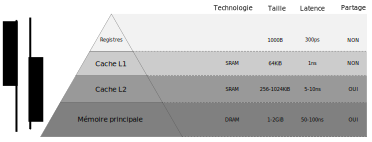
\includegraphics[width=\linewidth]{graphics/figures/hierarchie.pdf}
	\caption{\label{fig:hierarchie_memoire} Hiérarchie mémoire couramment rencontrée dans les terminaux mobiles}.
\end{figure}

Le niveau le plus bas de la hiérarchie mémoire est occupé par les registres, utilisés par le processeur pour le stockage des opérandes et des résultats intermédiaires.
Le niveau le plus haut est occupé par la mémoire principale basée sur la technologie DRAM.
Les niveaux intermédiaires sont occupés par les \emph{caches}, destinés à accélérer l'accès à la mémoire principale en stockant les données accédées récemment dans de la SRAM.
Cette architecture est conçue pour exploiter deux caractéristiques du comportement d'accès à la mémoire couramment observé dans les programmes: la localité spatiale~\cite{liptay1968structural} et la localité temporelle~\cite{wilkes1965slave}.
La propriété de localité spatiale exprime une forte probabilité que lorsqu'une donnée est accédée, les données voisines sont accédées dans un futur proche.
Tandis que la propriété de localité temporelle exprime une forte probabilité qu'une donnée accédée récemment le soit de nouveau dans un futur proche.
Dans les processeurs multicœurs, les niveaux supérieurs de cette hiérarchie sont généralement partagés, faisant des caches et de la mémoire principale d'éventuels canaux d'interférences.
Nous allons maintenant détailler le fonctionnement et l'impact des interférences sur ces deux composants.

\subsection{Mémoire principale}

La mémoire principale est implantée par des cellules de DRAM afin d'offrir une grande capacité de stockage.
L'utilisation de ce type de cellules apporte un certain nombre de contraintes, qui impose une organisation particulière que nous allons maintenant détailler.

\subsubsection{Organisation}

La mémoire principale est composée de modules (Dual Inline Memory Module ou DIMM) et de contrôleurs mémoires.
Un ensemble de modules mémoire est associé à un contrôleur mémoire par le biais d'un \emph{canal de communication ou channel}.
Ce canal est constitué de trois bus: un \emph{bus de commande}, un \emph{bus d'adresse}, et un \emph{bus de données}.
Le contrôleur reçoit des requêtes d'accès mémoires qu'ils décomposent en une série de commandes.
Les bus de commandes, d'adresses et de données sont alors utilisés respectivement pour transférer les commandes, les adresses de destination et les données lues ou écrites.

Un module mémoire comprend plusieurs \emph{puces mémoires} qui sont regroupées en ranks.
Une requête mémoire est émise à destination d'un rank en particulier, les puces qui le composent sont alors activées.
Les puces constituant un rank partagent le bus de commandes et d'adresse, mais occupent chacune une portion du bus de donnée.
Cela signifie que les données sont transférées en parallèle à partir de toutes les puces du rank, permettant ainsi de compenser la latence de la DRAM par une bande passante plus élevée.

Chaque puce est constitué de plusieurs \emph{bancs mémoires} ou plus rarement \emph{pages} (à ne pas confondre avec les pages de mémoire virtuelle).
Un banc mémoire comprend une matrice de cellules DRAM organisé en ligne et en colonne, plus une ligne supplémentaire appelée \emph{row buffer}.
Lorsque une donnée est accédée dans un banc mémoire, toute la ligne à laquelle elle appartient est chargée dans le row buffer.
Il y a deux raisons à cela.
D'une part, cela permet de gérer le fait que lire une cellule de DRAM détruit son contenu.
D'autre part, cela permet d'accélérer l'accès aux données présentes sur la même ligne.
Si la ligne à laquelle appartient une donnée auquelle on souhaite accéder n'est pas chargée, il y a alors \emph{un défaut de ligne ou row miss}.
Il faut alors écrire la ligne présente dans le row buffer (qu'elle ait été modifiée ou non) avant de charger la ligne désirée.

\begin{figure}
	\centering
	\includegraphics[width=\linewidth]{graphics/figures/orga-dram.pdf}
	\caption{\label{fig:dram_organization}Organisation de la mémoire principale}
\end{figure}
% \begin{figure}
% 	\centering
% 	\begin{tabular}{c c}
% 		\begin{subfigure}[t]{0,5\linewidth}
% 			\includegraphics[width=0.75\linewidth]{graphics/figures/dimm2.pdf}
% 			\caption{\label{fig:dimm}Modules mémoires}
% 		\end{subfigure} & 
	
% 		\begin{subfigure}[t]{0,5\linewidth}
% 			\includegraphics[width=0.75\linewidth]{graphics/figures/rank3.pdf}
% 			\caption{\label{fig:rank}Rank}
% 		\end{subfigure} \\
% 		& \\
% 		\begin{subfigure}[t]{0,3\linewidth}
% 			\includegraphics[width=\linewidth]{graphics/figures/chip2.pdf}
% 			\caption{\label{fig:rank}Puce mémoire}
% 		\end{subfigure} & 
		
% 		\begin{subfigure}[t]{0,3\linewidth}
% 			\includegraphics[width=\linewidth]{graphics/figures/bank2.pdf}
% 			\caption{\label{fig:bank}Banc mémoire} 
% 		\end{subfigure} \\
% 	\end{tabular}
% 	\caption{\label{fig:dram_organization}Organisation de la mémoire principale}
% \end{figure}

\subsubsection{Contrôleur DRAM}

Le contrôleur DRAM est en charge de traiter les différentes requêtes d'accès à la DRAM, tout en maintenant cette dernière dans un état de fonctionnement correct.
Il gère entre autres les différentes contraintes temporelles, dont le rafraichissement des cellules.
Le contrôleur reçoit des requêtes de lectures et d'écritures qu'il traduit en un ensemble de commandes agissant sur les bancs mémoires.
Plusieurs commandes sont définies par les JEDEC~\cite{specification2010jesd79}(l'organisation gérant les normes concernant la mémoire dynamique), parmi lesquels nous citerons les suivantes:

\begin{itemize}
	\item \texttt{ACT} charge une ligne dans le row buffer.
	\item \texttt{PRE} Vide le contenu du row buffer dans les cellules mémoire correspondantes.
	\item \texttt{READ} Lecture depuis le row buffer
	\item \texttt{WRITE} Écriture dans le row buffer
	\item \texttt{REF} Rafraichissement d'une ligne.
	Il s'agit de la combinaison d'une commande \texttt{ACT} et \texttt{PRE}.
	Cela a pour conséquence de vider le row buffer.
\end{itemize}

Les row buffers jouent un rôle essentiel dans la performance dans le DRAM.
Ils peuvent être gérés suivant deux politiques.
\begin{itemize}
	\item \emph{La politique open-row} Une ligne chargée dans un row buffer le reste jusqu'a son éviction.
	Cette stratégie est optimale pour les accès séquentiels.
	Par contre, le coût des défauts de lignes est élevé, étant donné qu'il faut écrire le contenu du row buffer avant de charger la nouvelle ligne.

	\item \emph{La politique close-row} La ligne est close après chaque accès.
	Cette politique offre un meilleur pire cas en évitant les conflits sur les row buffers, mais dégrade les performances en moyenne.
\end{itemize}

Le contrôleur mémoire est également en charge de maximiser les performances d'accès à la DRAM.
Pour cela, il réordonnance les requêtes d'accès afin de maximiser le débit de requêtes traitées et la bande passante de la mémoire principale.
La politique le plus couramment utilisée est \emph{Premier Prêt/Premier Arrivé Premier Servi ou FR/FCFS}.
Dans cette politique, les requêtes sont traitées dans l'ordre d'arrivée, mais une priorité est donnée à celle qui sont \emph{prête à être traitées}.
En pratique, une requête est prête à être traitée si la ligne correspondante est chargée, et si le bus de donnée est dans le bon sens (lecture ou écriture).
Le contrôleur optimise donc la bande passante globale aux dépens de l'équité des requêtes.

\begin{figure}[!h]
	\centering
	\begin{tabular} {c c}
		\begin{subfigure}[t]{0,4\linewidth}
			\centering
			\includegraphics[width=0.8\linewidth]{graphics/figures/open_row_policy_algo2.pdf}
			\caption{\label{fig:open_row_algo}Algorithme de la politique \emph{open-row}}
		\end{subfigure} & 
		
		\begin{subfigure}[t]{0,5\linewidth}
			\includegraphics[width=\linewidth]{graphics/figures/open_row_policy_wcet2.pdf}
			\caption{\label{fig:open_row_wcet}Pire cas de la politique \emph{open-row}}
		\end{subfigure} \\
		& \\
		\begin{subfigure}[t]{0,3\linewidth}
			\centering
			\includegraphics[width=0.6\linewidth]{graphics/figures/close_row_policy_algo2.pdf}
			\caption{\label{fig:closed_row_algo}Algorithme de la politique \emph{close-row}}
		\end{subfigure} &
		
		\begin{subfigure}[t]{0,5\linewidth}
			\includegraphics[width=\linewidth]{graphics/figures/close_row_policy_wcet2.pdf}
			\caption{\label{fig:closed_row_algo}Pire cas de la politique \emph{close row}}
		\end{subfigure} \\
	\end{tabular}

	\caption{\label{open_close_row}Algorithmes et pire cas des politiques de gestion de row buffer}
\end{figure}

\subsubsection{Mémoire principale et interférences}

La mémoire principale est un canal d'interférences spatiales et temporelles pour les différents cœurs qui l'utilisent.

Deux types de conflits peuvent survenir.
Les \emph{conflits de bancs} surviennent lorsque plusieurs cœurs tentent d'accéder au même banc mémoire simultanément.
Ce type de conflit est une interférence temporelle: il cause une séquentialisation des commandes.
Les \emph{conflits de lignes} surviennent lorsque deux commandes accèdent à deux lignes différentes sur le même banc, entrainant ainsi des rechargements de row buffer.
Il s'agit ici d'une interférence spatiale affectant la disponibilité des row buffers.
Ce type de conflits peut techniquement être évité en utilisant la politique close-row. 
Mais en pratique, c'est la politique open-row qui est employée, vu qu'elle permet d'atteindre de meilleures performances en moyenne.

La politique de réordonnancement de requête est une autre source d'interférence temporelle.
La politique FR/FCFS donne en effet la priorité aux requêtes d'accès pouvant être traitée immédiatement.
En conséquence, un cœur utilisant la DRAM efficacement, c'est-à-dire jouissant d'une bonne localité spatiale et temporelle, sera plus prioritaire qu'un cœur avec une utilisation moins efficace.
On peut en conclure que l'iniquité de cette politique rend plus sensibles aux interférences sur la mémoire principale les applications l'utilisant de façon non optimale.

% \begin{keypoints}
% 	\item Les caches jouent un rôle majeur dans la performance des processeurs modernes en masquant la latence d'accès à la mémoire.
% 	\item Les caches partagées constituent un canal d'interférences aussi bien spatiales que temporelles.
% \end{keypoints}

\subsection{Caches}

Les caches ont pour but de réduire la latence moyenne d'accès à la mémoire.
Pour cela, ils stockent un sous-ensemble des données présentes en mémoire dans une mémoire SRAM, qui est donc très rapide, mais de taille limitée.
En stockant les données accédées récemment, ils permettent de considérablement améliorer les performances des programmes présentant une bonne localité spatiale et temporelle.
En effet, comme on peut le constater dans la figure~\ref{fig:hierarchie_memoire}, la latence d'accès à la mémoire principale peut atteindre l'ordre de la centaine de nanosecondes contre une nanoseconde pour un accès au cache de niveau un.
Les caches sont donc un élément crucial pour la performance des processeurs modernes.

\subsubsection{Accès}

L'accès au cache est complètement transparent pour le programmeur.
Lorsqu'une donnée est accédée, le cache de plus bas niveau est d'abord interrogé sur sa présence.
Si la donnée est présente dans le cache, elle est alors accédée en lecture ou écriture depuis celui-ci.
Dans le cas contraire, la donnée doit alors être chargée depuis le niveau suivant de la hiérarchie mémoire, on parle alors de \emph{défaut de cache ou cache miss}.
Le niveau suivant de la hiérarchie mémoire peut alors être directement la mémoire principale, ou bien un autre cache.
Nous pouvons distinguer quatre types de défauts de caches:

\begin{itemize}
	\item \emph{Défauts obligatoires} La donnée est chargée pour la première fois.
	\item \emph{Défauts capacitifs} Le cache est plein, la donnée doit alors être chargée aux dépens d'une autre.
	\item \emph{Défauts conflictuels} deux données distinctes partagent le même emplacement de cache et s'évincent mutuellement.
	\item \emph{Défauts de cohérence} La donnée a été invalidée par un protocole de cohérence.
\end{itemize}

\subsubsection{Organisation}

Un cache est divisé en \emph{blocs} appelés \emph{lignes}.
Une ligne de cache comprend plusieurs mots mémoires (généralement huit).
Les transferts de données se font à la granularité du mot mémoire vers le processeur, et à la granularité de la ligne de cache vers les autres niveaux de la hiérarchie mémoire.
Des métadonnées sont associées à chaque ligne de cache, leur nature exacte pouvant varier légèrement d'un type de cache à l'autre.

Le placement des données dans le cache se fait au moyen de l'adresse de la donnée accédée.
Cette dernière contient trois informations essentielles: 
\begin{itemize}
	\item \emph{L'index} désigne un sous-ensemble de lignes de caches pouvant accueillir la donnée.
	\item \emph{L'offset} désigne la position d'un octet dans la ligne de cache.
	\item \emph{Le tag} permet de déterminer l'adresse de la donnée présente dans une ligne.
\end{itemize}

La position des bits encodant cette information est décrite dans la figure~\ref{fig:addresse_cache}.
Le découpage choisi n'est pas anodin.
Il associe aux lignes adjacentes en mémoire des index adjacents dans le cache, prévenant ainsi des défauts conflictuels pour les applications jouissant d'une bonne localité spatiale.

\begin{figure}[!h]
	\centering
	\includegraphics[width=0.9\linewidth]{graphics/figures/cache-adresse.pdf}
	\caption{\label{fig:addresse_cache}Correspondance entre les bits d'adresses et le placement des données dans un cache}
\end{figure}

On peut utiliser aussi bien l'adresse virtuelle que l'adresse physique pour tagger et indexer le cache.
On rencontre trois cas:
\begin{itemize}
	\item \emph{Cache Virtuellement Indexé et Virtuellement Taggé (VIVT)}
	Seule l'adresse virtuelle est utilisée pour interroger le cache.
	Cette méthode a l'avantage de la rapidité, vu qu'elle ne nécessite pas de traduire l'adresse.
	Elle pose néanmoins le problème des homonymes, deux mêmes adresses virtuelles pouvant désigner deux emplacements physiques différents.
	Ce problème a d'autant plus de chance de survenir dans le cas où le cache est partagé.
	Si des solutions à ce problème existent, elles se révèlent incompatibles avec les protocoles de cohérences de caches classiques~\cite{Kaxiras:2013:NPE:2485922.2485968}.

	\item \emph{Cache Physiquement Indexé et Physiquement Taggé (PIPT)}
	Seule l'adresse physique est utilisée.
	Cette méthode permet d'éviter le problème des homonymes, mais présente l'inconvénient de la lenteur, une traduction de l'adresse étant nécessaire pour interroger le cache.

	\item \emph{Cache Virtuellement Indexé et Physiquement Taggé (VIPT)}
	Cette approche vise à réduire le temps d'accès au cache en accédant à la ligne à tester pendant la traduction de l'adresse.
	L'utilisation de l'adresse physique permet d'éviter les problèmes d'homonymies.
	Pour cela, il faut néanmoins qu'il n'y ait aucun bit d'index ne soit traduit, ce qui limite cette approche aux caches de petite taille.
\end{itemize}

\subsubsection{Politiques de correspondance}

La politique de correspondance d'un cache définit quelle ligne peut être occupée pour un index donné.

Si un index ne désigne qu'une seule ligne dans le cache, celui-ci est dit à \emph{correspondance préétablie (direct mapped)} (figure~\ref{fig:direct_mapping}).
Cette politique a l'avantage d'être peu coûteuse à mettre en œuvre.
En effet, lorsque le cache est interrogé, il suffit de tester une seule ligne.
Elle a par contre l'inconvénient d'être à l'origine de nombreux défauts conflictuels.

La politique réciproque est de faire correspondre n'importe quelle ligne du cache pour un index donné.
Un cache utilisant cette politique est alors dit \emph{pleinement associatif ou full associative} (figure~\ref{fig:full_assoc}).
Lors des défauts capacitaires, une \emph{politique de remplacement} est appliquée afin de déterminer quelle ligne va être remplacée.
Différentes politiques de remplacement peuvent être appliquées: \emph{FIFO}, \emph{aléatoire}, \emph{Least Recently Used}.
Si cette politique de correspondance offre une flexibilité optimale à la politique de remplacement, elle nécessite également de tester toutes les lignes de caches lorsque le cache est interrogé, ce qui se traduit par des coûts d'implantations prohibitifs.

La politique de correspondance utilisée en pratique est \emph{l'association partielle ou set associativity} (figure~\ref{fig:set_assoc}).
Il s'agit d'un compromis entre la correspondance préétablie et la pleine association.
Cette politique associe à chaque index un ensemble de taille fixe de lignes.
En cas de défaut capacitif, la politique de remplacement choisit la ligne à remplacer parmi les lignes de l'ensemble correspondant.
Le cache est alors divisé en \emph{voies ou cache ways} correspondant aux différents emplacements d'un ensemble de lignes.
\emph{L'associativité} désigne la taille des ensembles de lignes, et donc le nombre de voies du cache.
On peut voir un cache à correspondance préétablie comme un cache partiellement associatif avec une seule voie.
De même, un cache pleinement associatif peut être vu comme un cache partiellement associatif ne comportant qu'un seul ensemble de lignes. 

\begin{figure}[!h]
	\begin{subfigure}[t]{0.5\linewidth}
		\includegraphics[width=\linewidth]{graphics/figures/cache-direct-mapping.pdf}
		\caption{\label{fig:direct_mapping}Association directe}
	\end{subfigure}
	\begin{subfigure}[t]{0.5\linewidth}
		\includegraphics[width=\linewidth]{graphics/figures/cache-full-assoc.pdf}
		\caption{\label{fig:full_assoc}Associativité totale}
	\end{subfigure}
	\begin{subfigure}[b]{0.5\linewidth}
		\includegraphics[width=\linewidth]{graphics/figures/cache-set-assoc.pdf}
		\caption{\label{fig:set_assoc}Associativité partielle}
	\end{subfigure}
	\caption{\label{fig:indexation_associativité} Politiques de correspondances}
\end{figure}

\subsubsection{Politiques d'écritures}

La politique d'écriture d'un cache détermine quand les données sont écrites vers le niveau supérieur.
On en dénombre deux:

\begin{itemize}
	\item \emph{Écriture directe (Write Through)} Les écritures sont immédiatement propagées vers le niveau supérieur.
	Cette politique a l'avantage de simplifier la maintenance de la cohérence entre les différents niveaux de la hiérarchie mémoire; au prix, néanmoins d'une plus grande consommation de bande passante.
	
	\item \emph{Écritures différées (Write Back)} Les données ne sont écrites vers le niveau supérieur que lors de leur remplacement.
	Les métadonnées des lignes des caches utilisant cette politique comprennent un bit \emph{dirty}, qui est activé lorsque les données de la ligne sont modifiées.
	Lors du remplacement d'une ligne, le bit dirty est d'abord testé.
	La donnée n'est alors écrite en mémoire que dans le cas où ce dernier a été activé.
	Cette politique permet de réduire le trafic vers les niveaux supérieurs de la hiérarchie mémoire, mais elle complexifie également la gestion de la cohérence des données.
\end{itemize}

\subsubsection{Politiques d'allocation}

La politique d'allocation détermine si une donnée chargée depuis le niveau de cache supérieur doit être copiée dans le cache (\emph{line fill}) ou non.
Il y a deux politiques d'allocations:

\begin{itemize}
	\item \emph{Read-allocate} Un line fill n'est effectué que lors des défauts de cache en lecture.
	Lors d'un défaut de cache en écriture, le cache n'est pas modifié et l'écriture transmise au niveau supérieur.
	\item \emph{La politique write-allocate} Un line fill a lieu lors des défauts de caches en lecture et en écriture.
	Cette politique est généralement utilisée dans les caches \emph{write-back}.
\end{itemize}

\subsubsection{Caches et interférences}

Les caches partagés sont des canaux d'interférences importants dans les processeurs modernes.
Elles peuvent être aussi bien spatiales que temporelles.
Elles entrainent trois effets indésirables majeurs:

\begin{itemize}
	\item \emph{Interférence temporelle lors de l'accès au cache} Les caches ont la capacité de traiter plusieurs accès en parallèle.
	Cette capacité peut néanmoins être excédée lors de l'utilisation en simultané du cache par plusieurs cœurs.
	Dans ce cas, des requêtes ayant dû être traitées en parallèle le sont séquentiellement induisant une latence supplémentaire.
	
	\item \emph{Contention inter-cœurs sur les lignes de cache} Les lignes de caches d'une application s'exécutant sur un cœur peuvent être remplacée au profit des lignes d'une application sur un autre cœur, ce qui a pour conséquence une augmentation des défauts conflictuels.
	Ces interférences spatiales, dites inter-cœur, ont un impact considérable sur les pires temps d'exécution, se traduisant par un surdimensionnent inacceptable du matériel.

	\item \emph{Interférence spatiale causée par les protocoles de cohérences} Lorsque des données sont partagées entre les cœurs, il faut maintenir la cohérence entre les différents caches du système.
	Les protocoles utilisés pour maintenir cette cohérence peuvent \emph{invalider} des données, provoquant ainsi une augmentation des défauts de cohérences.
	Ce problème touche surtout les systèmes adoptant le modèle symétrique.

\end{itemize}

\section{Conclusions du chapitre}

Dans cette section, nous avons présenté le problème des interférences dans les processeurs multi-cœurs destinés au marché de masse.
Ces interférences, dues aux accès concurrents aux ressources partagés entre les cœurs, sont la source de ralentissement pour des applications, empêchant ainsi l'isolation temporelle requise pour garantir la sûreté des systèmes intégrés temps-réel.
Ce problème concerne notamment le système mémoire, qui est à ce jour l'un des principaux acteurs de la performance des processeurs modernes.

% Conclusions: système embarqués => arhitecture intégrées => besoin de garantir le déterminisme => isolation temporelle

% 			pb interférence du aux partages de ressources matérielle.
% 			Principal canaux d'interférence situés dans le chemin d'accès à la mémoire
% 			Cache et DRAM concerné. Aussi bien vol de ressources qu'arbitrage.

% Transition : Interférences temporelle => pb en temps-réel. Plus de détail sur ces systèmes + approches proposée pour gérer ce problème.

Les interférences sont un problème, car elles peuvent causer la défaillance des applications temps-réel du système.
Dans le chapitre suivant, nous allons nous pencher plus en détail sur les aspects temps-réel et l'impact des interférences sur ces derniers.
Nous y présenterons également les approches proposées par la communauté scientifique pour apporter une solution au problème des interférences.